\documentclass{beamer}
\usetheme{Juelich}

\title{Quantum Boltzmann Machines}
\subtitle{Applications in Finance}
\author{Cameron Perot}
\institute{JSC}
\date{\today}
\titlegraphic{\includegraphics%
    [height=0.45\paperheight]{placeholder}
}

% packages
\usepackage{amssymb}
\usepackage{amsmath}
\usepackage{float}
\usepackage{graphicx}
\usepackage{braket}
\usepackage{multirow}
\usepackage{bbm}
\usepackage{mathtools}

\graphicspath{ {../../../artifacts/BernoulliRBM_20211104_202501/plots/}{../../../results/plots/data_analysis/}{../../images/} }

% new commands
% Misc. commands
\newcommand{\CNOT}[2]{\text{C}_{#1}\text{NOT}_{#2}}
\newcommand{\SWAP}{\text{SWAP}}
\newcommand{\CZ}{\text{CZ}}
\newcommand{\tr}{\text{tr}}
\newcommand{\frt}{\frac{1}{\sqrt{2}}}
\newcommand{\Z}{\mathbb{Z}}
\newcommand{\R}{\mathbb{R}}
\newcommand{\N}{\mathbb{N}}
\newcommand{\mat}[1]{\mathbf{#1}}
\newcommand{\binset}{\{0,1\}}
\newcommand{\spause}{s_{\text{pause}}}
\newcommand{\tpause}{t_{\text{pause}}}
\newcommand{\Deltapause}{\Delta_{\text{pause}}}
\newcommand{\Deltaquench}{\Delta_{\text{quench}}}
\newcommand{\alphaquench}{\alpha_{\text{quench}}}
\renewcommand{\vec}[1]{\mathbf{#1}}
\newcommand{\basistwo}{\{\ket{00}, \ket{01}, \ket{10}, \ket{11}\}}
\DeclarePairedDelimiter{\norm}{\lVert}{\rVert}
\DeclarePairedDelimiter{\abs}{\lvert}{\rvert}

% Identity operator (on K^2)
\newcommand{\idtwo}{
    \begin{bmatrix}
        1 & 0 \\
        0 & 1
    \end{bmatrix}
}

% Hadamard operator
\newcommand{\Hgate}{
    \frac{1}{\sqrt{2}} \begin{bmatrix}
        1 & 1 \\
        1 & -1
    \end{bmatrix}
}

% T gate
\newcommand{\Tgate}{
    \begin{bmatrix}
        1 & 0 \\
        0 & e^{i \pi / 4}
    \end{bmatrix}
}

% T gate dag
\newcommand{\Tgatedag}{
    \begin{bmatrix}
        1 & 0 \\
        0 & e^{-i \pi / 4}
    \end{bmatrix}
}

% R_X
\newcommand{\RXGate}[1]{
    \begin{bmatrix}
        \cos\frac{#1}{2} & -i\sin\frac{#1}{2} \\
        -i\sin\frac{#1}{2} & \cos\frac{#1}{2}
    \end{bmatrix}
}

% R_Y
\newcommand{\RYGate}[1]{
    \begin{bmatrix}
        \cos\frac{#1}{2} & -\sin\frac{#1}{2} \\
        \sin\frac{#1}{2} & \cos\frac{#1}{2}
    \end{bmatrix}
}

% R_Z
\newcommand{\RZGate}[1]{
    \begin{bmatrix}
        e^{-i{#1}/2} & 0 \\
        0 & e^{i{#1}/2}
    \end{bmatrix}
}

% Pauli X operator
\newcommand{\XGate}{
    \begin{bmatrix}
        0 & 1 \\
        1 & 0
    \end{bmatrix}
}

% Pauli Y operator
\newcommand{\YGate}{
    \begin{bmatrix}
        0 & -i \\
        i & 0
    \end{bmatrix}
}

% Pauli Z operator
\newcommand{\ZGate}{
    \begin{bmatrix}
        1 & 0 \\
        0 & -1
    \end{bmatrix}
}

% The |0⟩ state in vector form
\newcommand{\zerostate}{
    \begin{bmatrix}
        1 \\
        0
    \end{bmatrix}
}

% The |1⟩ state in vector form
\newcommand{\onestate}{
    \begin{bmatrix}
        0 \\
        1
    \end{bmatrix}
}

% The |-⟩ state in vector form
\newcommand{\minusstatey}{
    \frac{1}{\sqrt{2}}
    \begin{bmatrix}
        1 \\
        -i
    \end{bmatrix}
}

% The |+⟩ state in vector form
\newcommand{\plusstatey}{
    \frac{1}{\sqrt{2}}
    \begin{bmatrix}
        1 \\
        i
    \end{bmatrix}
}

% The |-'⟩ state in vector form
\newcommand{\minusstate}{
    \frac{1}{\sqrt{2}}
    \begin{bmatrix}
        1 \\
        -1
    \end{bmatrix}
}

% The |+'⟩ state in vector form
\newcommand{\plusstate}{
    \frac{1}{\sqrt{2}}
    \begin{bmatrix}
        1 \\
        1
    \end{bmatrix}
}


\begin{document}
%----------------------------------------------------------------------------------------
% Title Page
%----------------------------------------------------------------------------------------

\maketitle

%----------------------------------------------------------------------------------------
% Table of Contents
%----------------------------------------------------------------------------------------

\begin{frame}
    \frametitle{Overview}
    \tableofcontents
\end{frame}

%----------------------------------------------------------------------------------------
% Restricted Boltzmann Machines
%----------------------------------------------------------------------------------------

\section{Restricted Boltzmann Machines}

\begin{frame}
    \frametitle{Restricted Boltzmann Machine (RBM)}
    \begin{figure}
        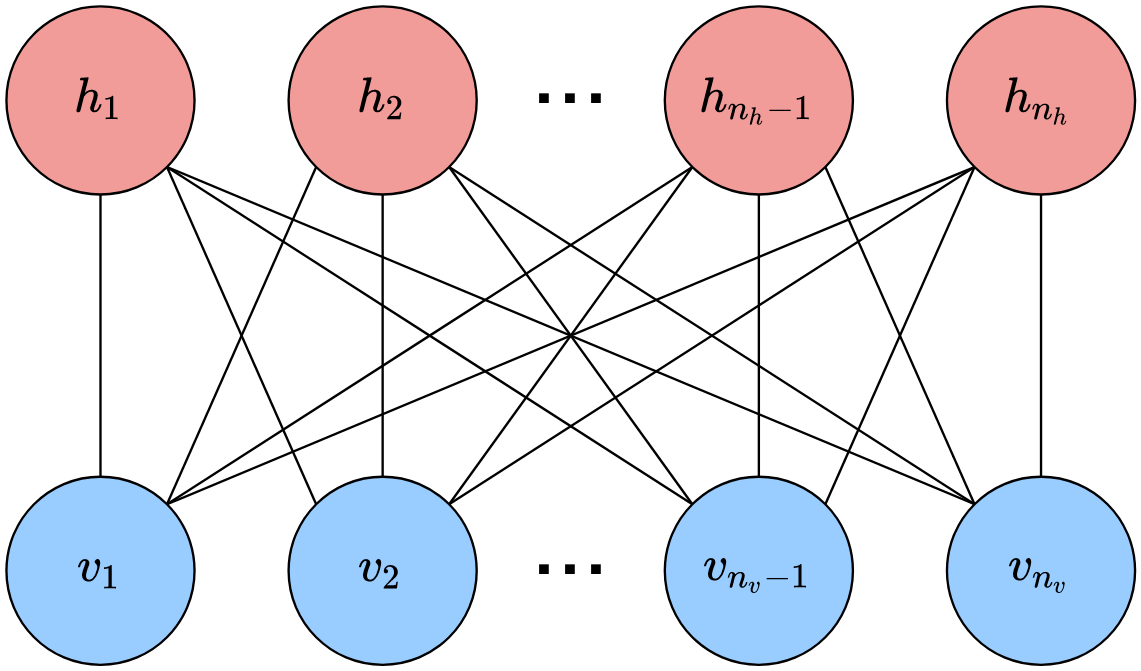
\includegraphics[width=0.8\linewidth]{rbm_diagram.png}
        \label{rbm_diagram}
        \caption{Bernoulli RBM, \( v_i \in \{0, 1\}, \ h_j \in \{0, 1\} \)}
    \end{figure}
\end{frame}

\begin{frame}
    \frametitle{Energy-Based Model}
    Energy function
    \[
        E(\mathbf{v}, \mathbf{h}) = -\sum_i a_i v_i - \sum_j b_j h_j - \sum_{i,j} w_{i,j} v_i h_j
    \]
    with joint probability given by
    \[
        p(\vv, \hv) = \frac{1}{Z} e^{-E(\vv, \hv)}
    \]
    and (intractable~\cite{long_servedio_2010}) partition function
    \[
        Z = \sum_{\vv,\hv} e^{-E(\vv, \hv)}
    \]
\end{frame}

\begin{frame}
    \frametitle{Conditional Probabilities}
    Due to the independence of units within the same layer, the conditional probabilities of the layers are given by~\footnote{Derivation can be found in~\cite{goodfellow_deep_learning} p. 658}
    \begin{align*}
        p(\hv | \vv) = \prod_j p(h_j | \vv) \\
        p(\vv | \hv) = \prod_i p(v_i | \hv)
    \end{align*}
    where~\footnote{\( \sigma(x) = \frac{1}{1 + e^{-x}} \) (logistic function) \\}
    \begin{align*}
        p(h_j = 1 | \vv) = \sigma\bigg( b_j + \sum_i w_{i,j} v_i \bigg) \\
        p(v_i = 1 | \hv) = \sigma\bigg( a_i + \sum_j w_{i,j} h_j \bigg)
    \end{align*}
\end{frame}

\begin{frame}
    \frametitle{Gibbs Sampling}
    \begin{itemize}
        \item Sampling from a trained model is done using Gibbs sampling (MCMC method), i.e., alternating between sampling \( \hv \) using \( p(\hv | \vv) \) and sampling \( \vv \) using \( p(\vv | \hv) \).
        \item Markov chain \( \rightarrow \) autocorrelations.
        \item Not necessarily efficient due to thermalization requirements.
    \end{itemize}
\end{frame}

\begin{frame}
    \frametitle{Training via Contrastive Divergence}
    Want to maximize the likelihood (i.e. minimize the negative log-likelihood).
    This can be done using stochastic gradient descent~\cite{hinton_rbm_training}, with
    \[
        \frac{\partial \log p(\vv)}{\partial w_{i,j}} = \langle v_i h_j \rangle_{\text{data}} - \langle v_i h_j \rangle_{\text{model}}
    \]

    \( \langle v_i h_j \rangle_{\text{model}} \) is nontrivial to obtain, so in practice this is (crudely) approximated using Gibbs sampling, leading to an iterative update of
    \[
        \Delta w_{i,j} = \eta (\langle v_i h_j \rangle_{\text{data}} - \langle v_i h_j \rangle_{\text{reconstructed}})
    \]
    where \( \eta \) is the learning rate hyperparameter
\end{frame}

%----------------------------------------------------------------------------------------
% Data Analysis
%----------------------------------------------------------------------------------------

\section{Data Analysis}

\begin{frame}
    \frametitle{Generative Modeling in Finance}
    \begin{itemize}
        \item Accurate generative modeling is important in risk management.
        \item A lot of modeling is done using Gaussian distribution based methods, some with mechanism for manually incorporating additional tail risk.
        \item Forex markets have a daily volume of \$6.6T~\cite{bis_2019}, the majority of which is concentrated in a few major pairs, e.g. EUR/USD, USD/JPY, GBP/USD, and USD/CAD.
        \item The raw data used in the following is sourced from Dukascopy\footnote{\href{https://www.dukascopy.com/plugins/fxMarketWatch/?historical_data}{https://www.dukascopy.com/plugins/fxMarketWatch/?historical\_data} \\} for the time period 1999-2019.
    \end{itemize}
\end{frame}

\begin{frame}
    \frametitle{EURUSD}
    \begin{figure}
        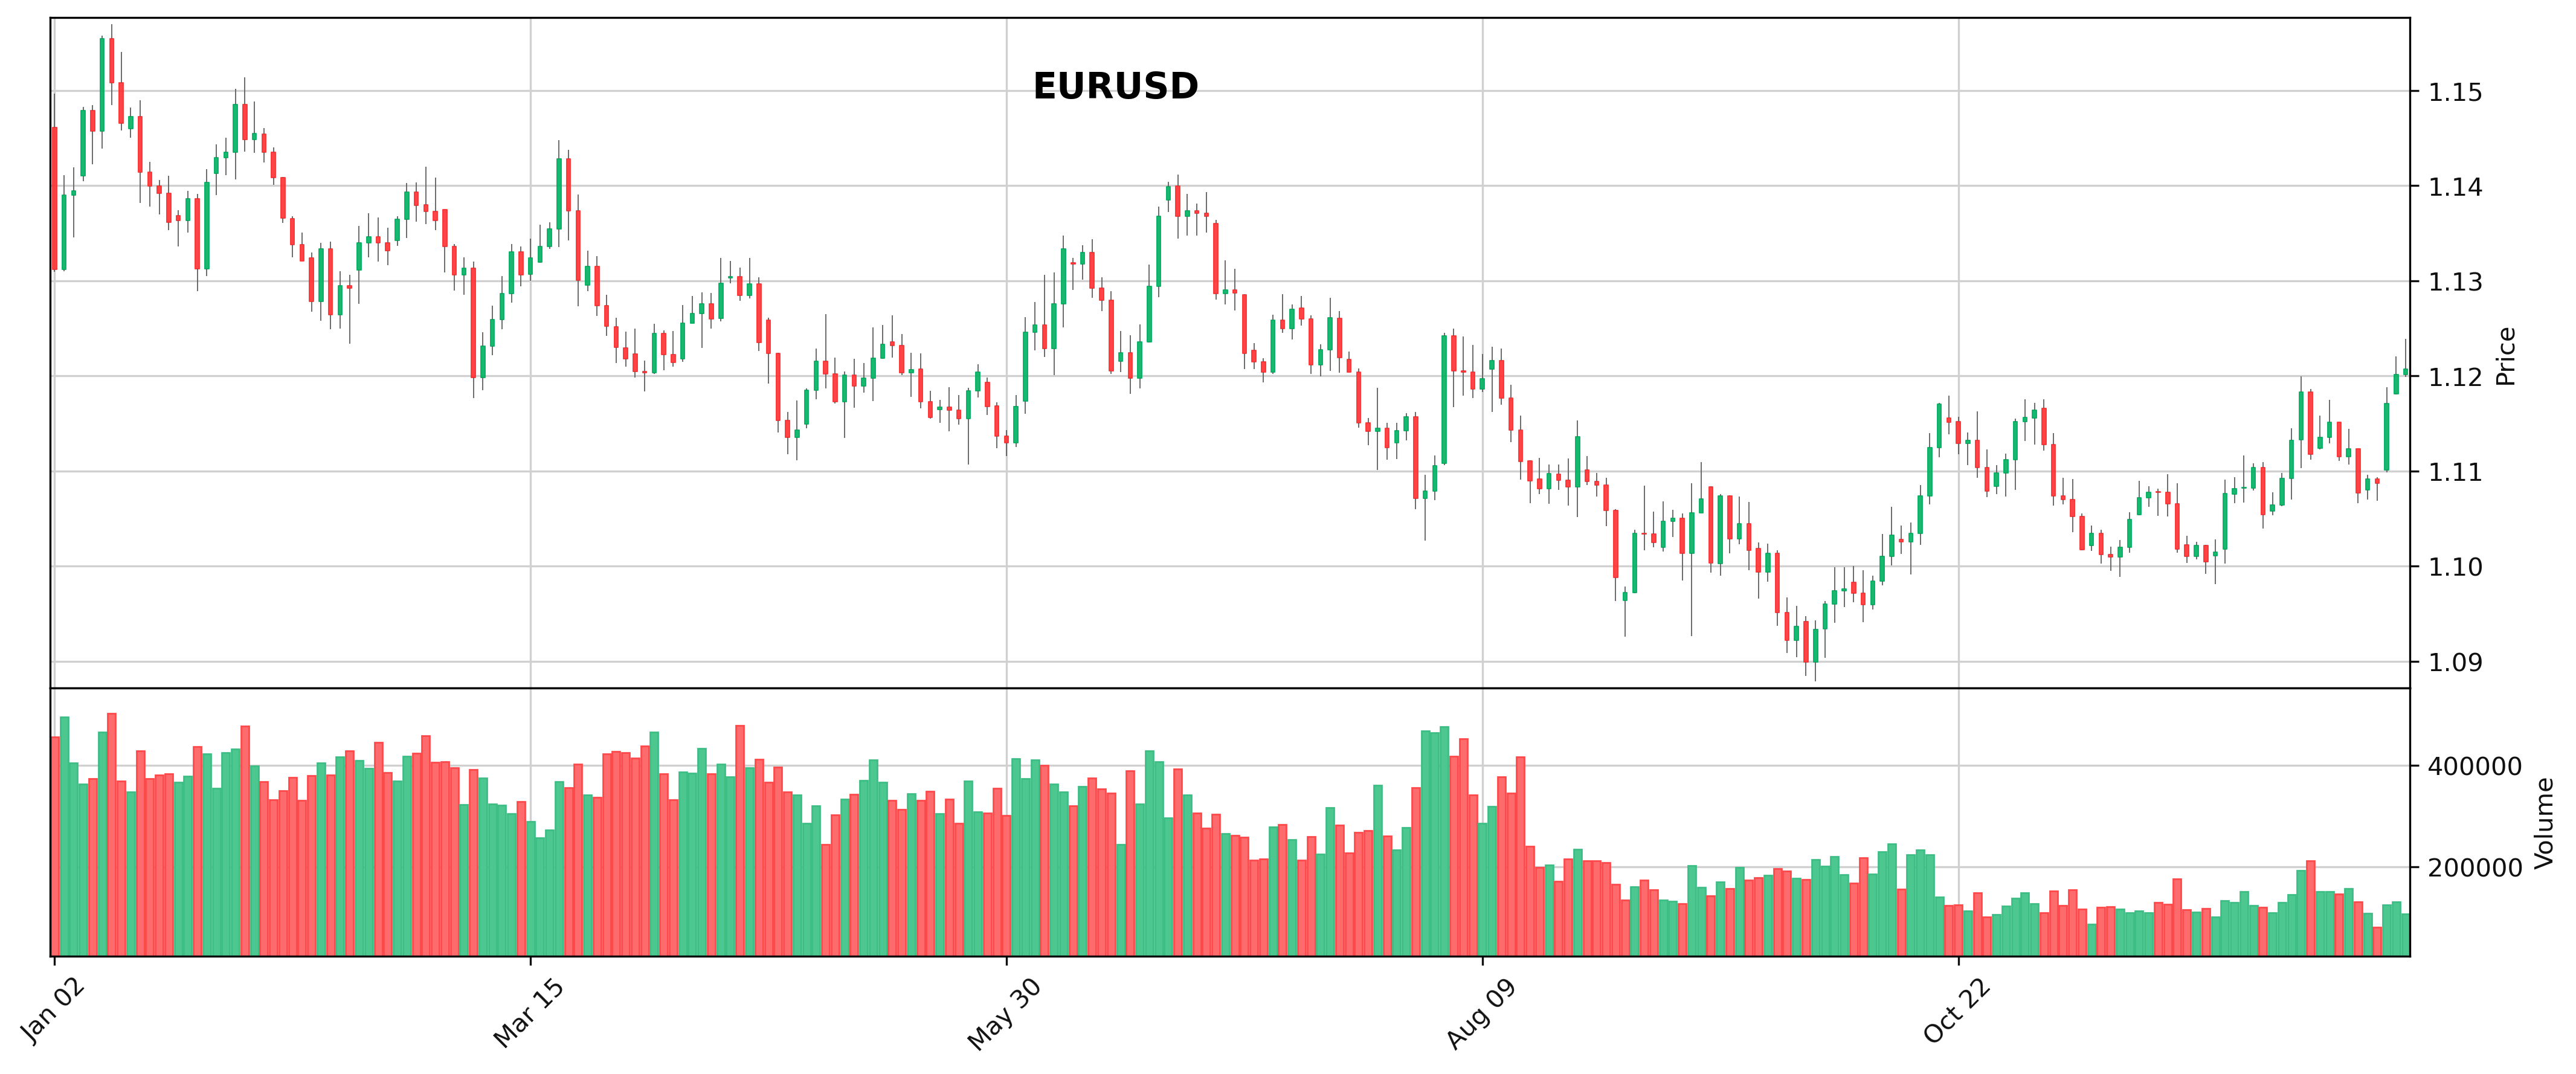
\includegraphics[width=1\linewidth]{candlestick_EURUSD.png}
        \label{EURUSD}
        \caption{EURUSD daily candlestick chart during 2019.}
    \end{figure}
\end{frame}

\begin{frame}
    \frametitle{Daily Log Returns~\footnote{\href{https://quantivity.wordpress.com/2011/02/21/why-log-returns/}{https://quantivity.wordpress.com/2011/02/21/why-log-returns/} \\} Histograms}
    \begin{figure}
        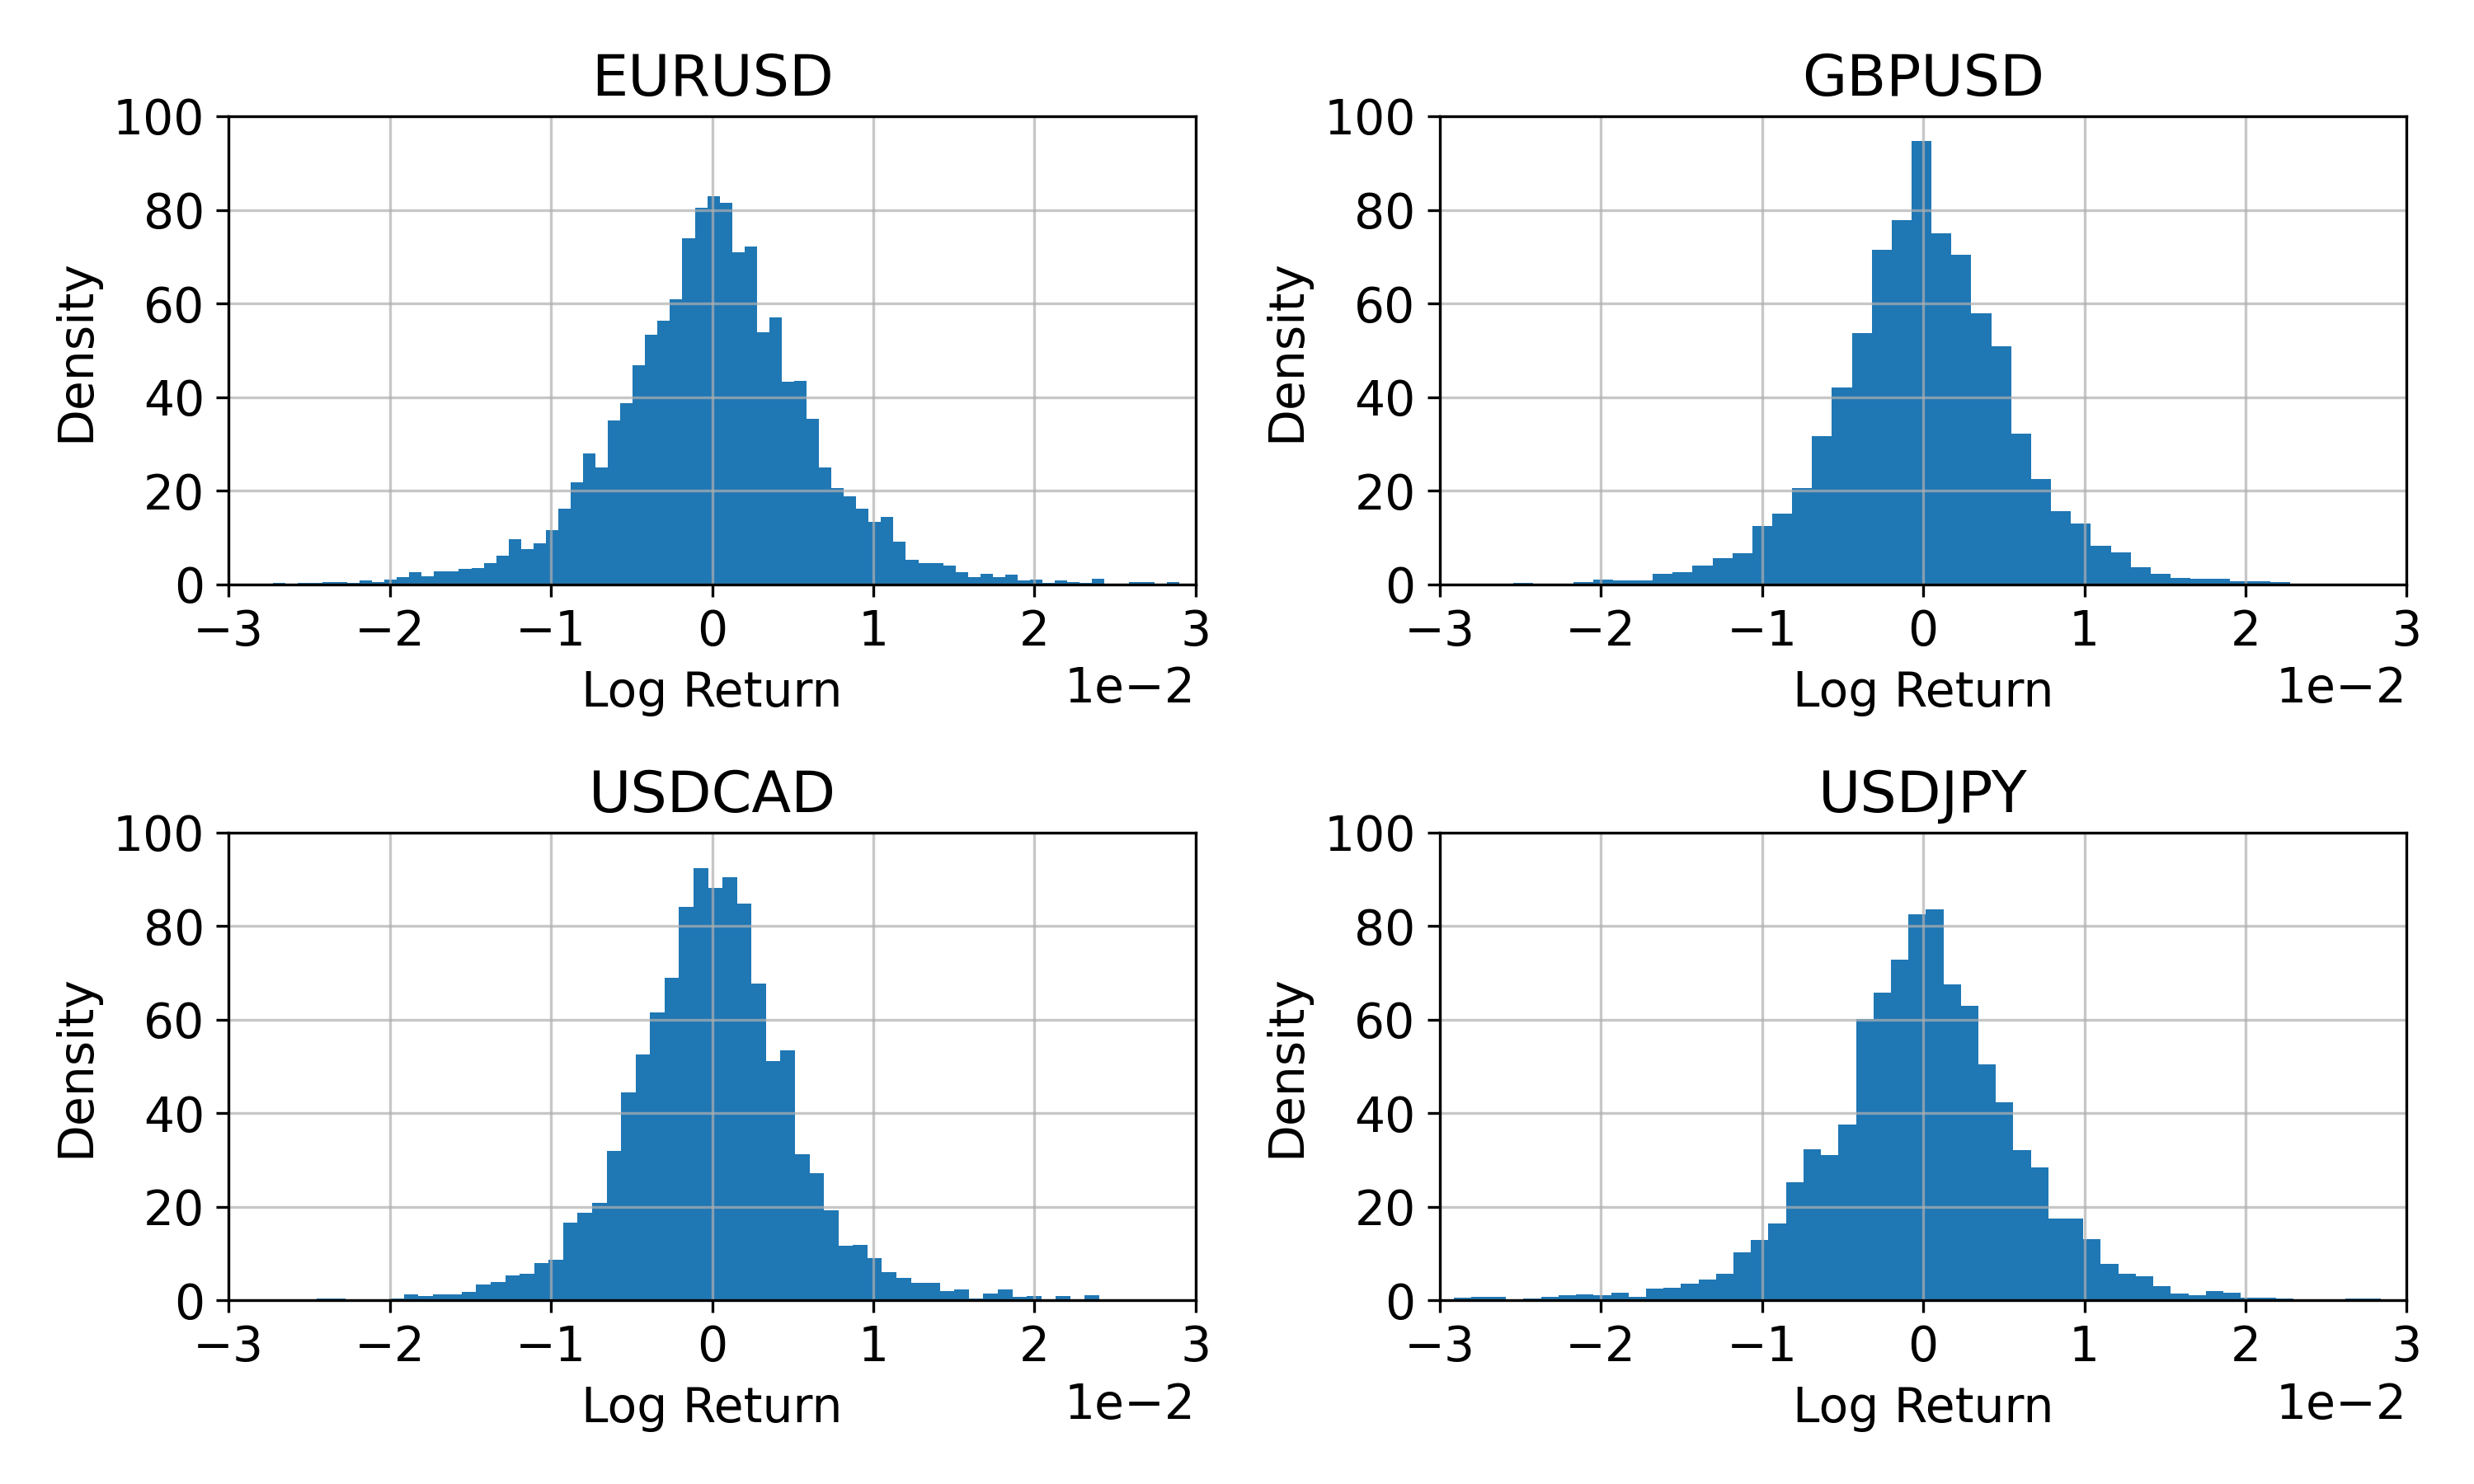
\includegraphics[width=0.9\linewidth]{histograms.png}
        \label{histograms}
    \end{figure}
\end{frame}

\begin{frame}
    \frametitle{Violin \& Box Plot}
    \begin{figure}
        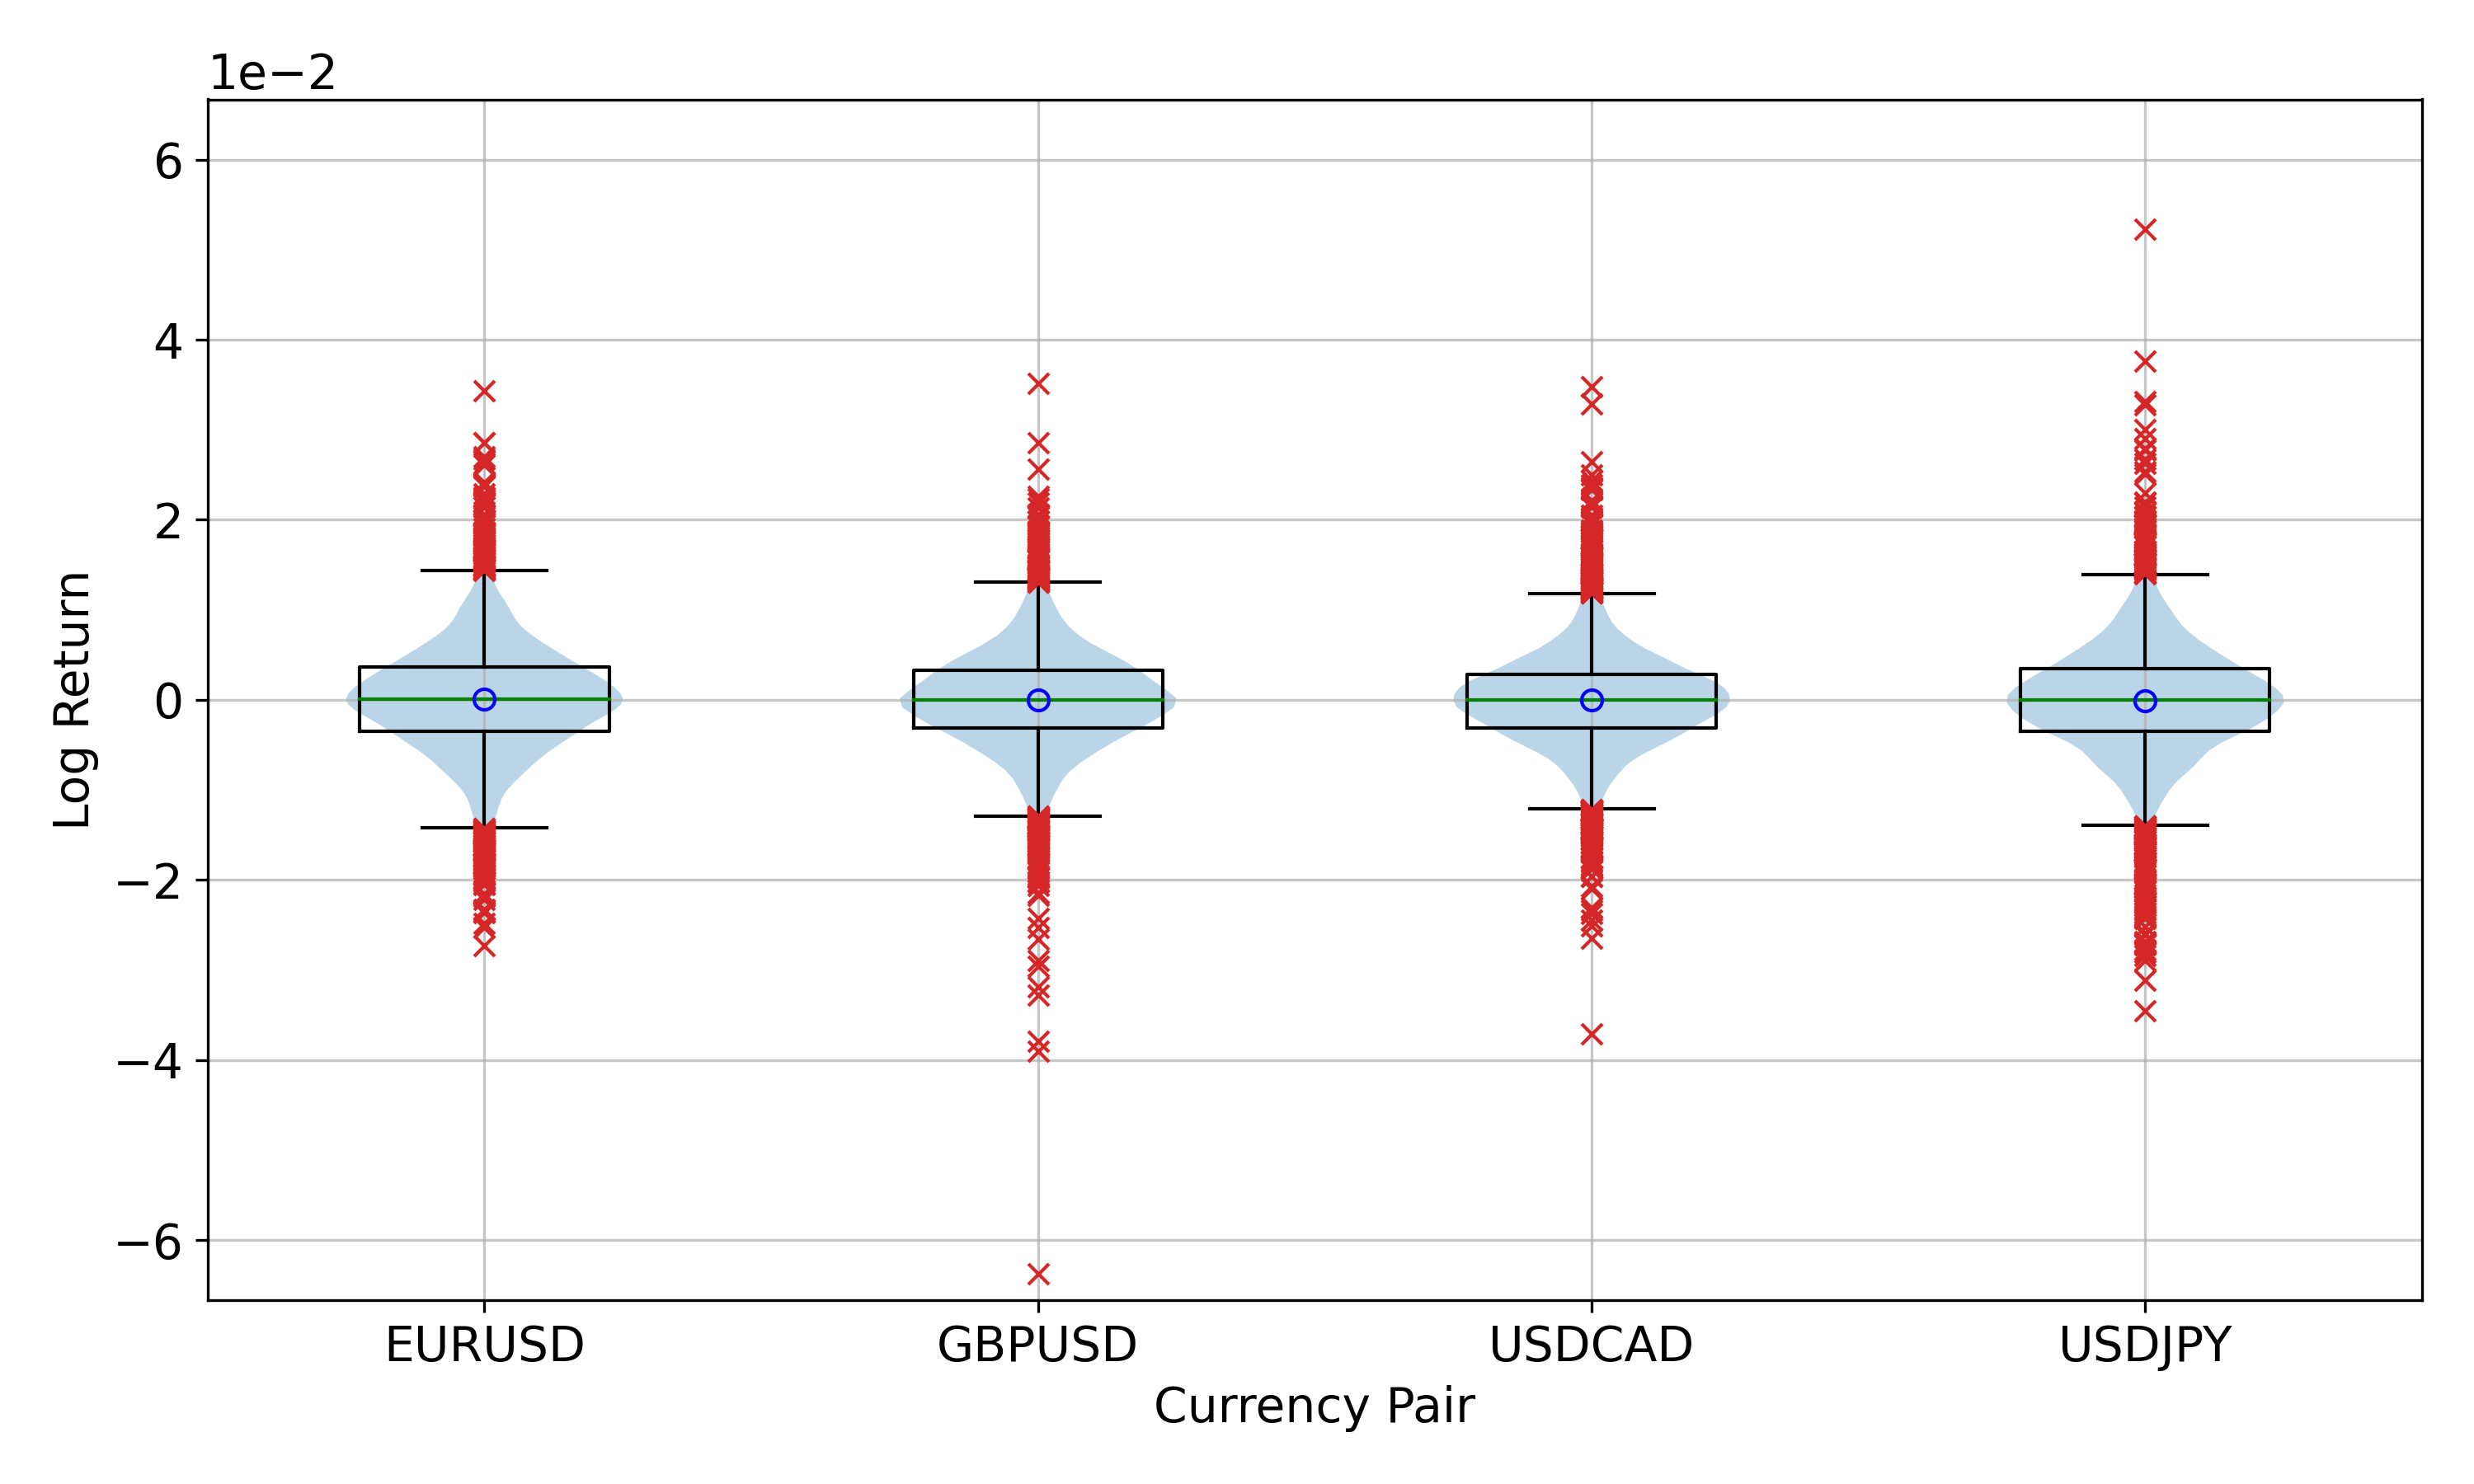
\includegraphics[width=0.9\linewidth]{violin.png}
        \label{violin}
    \end{figure}
\end{frame}

%----------------------------------------------------------------------------------------
% Classical RBM Modeling
%----------------------------------------------------------------------------------------

\section{Classical RBM Modeling}

\begin{frame}
    \frametitle{Adapting the Problem to an RBM}
    \begin{itemize}
        \item Log returns for each currency are linearly binarized into 16-bit vectors, and concatenated into a 64-bit vector for input into the RBM.
        \item The RBM has 30 hidden units.
        \item Trained with an initial learning rate of \( 10^{-3} \), and follows an exponential decay beginning after a predefined number of epochs.
        \item Trained with a minibatch size of 10.
        \item Ability to handle additional binary indicators, e.g. volatility regime (following results do not include additional binary indicators).
        \item Results are of the format \( \mu \pm \sigma \), from an ensemble of size 100.
    \end{itemize}
\end{frame}

%\begin{frame}
    %\frametitle{Rolling Volatilities}
    %\begin{figure}
        %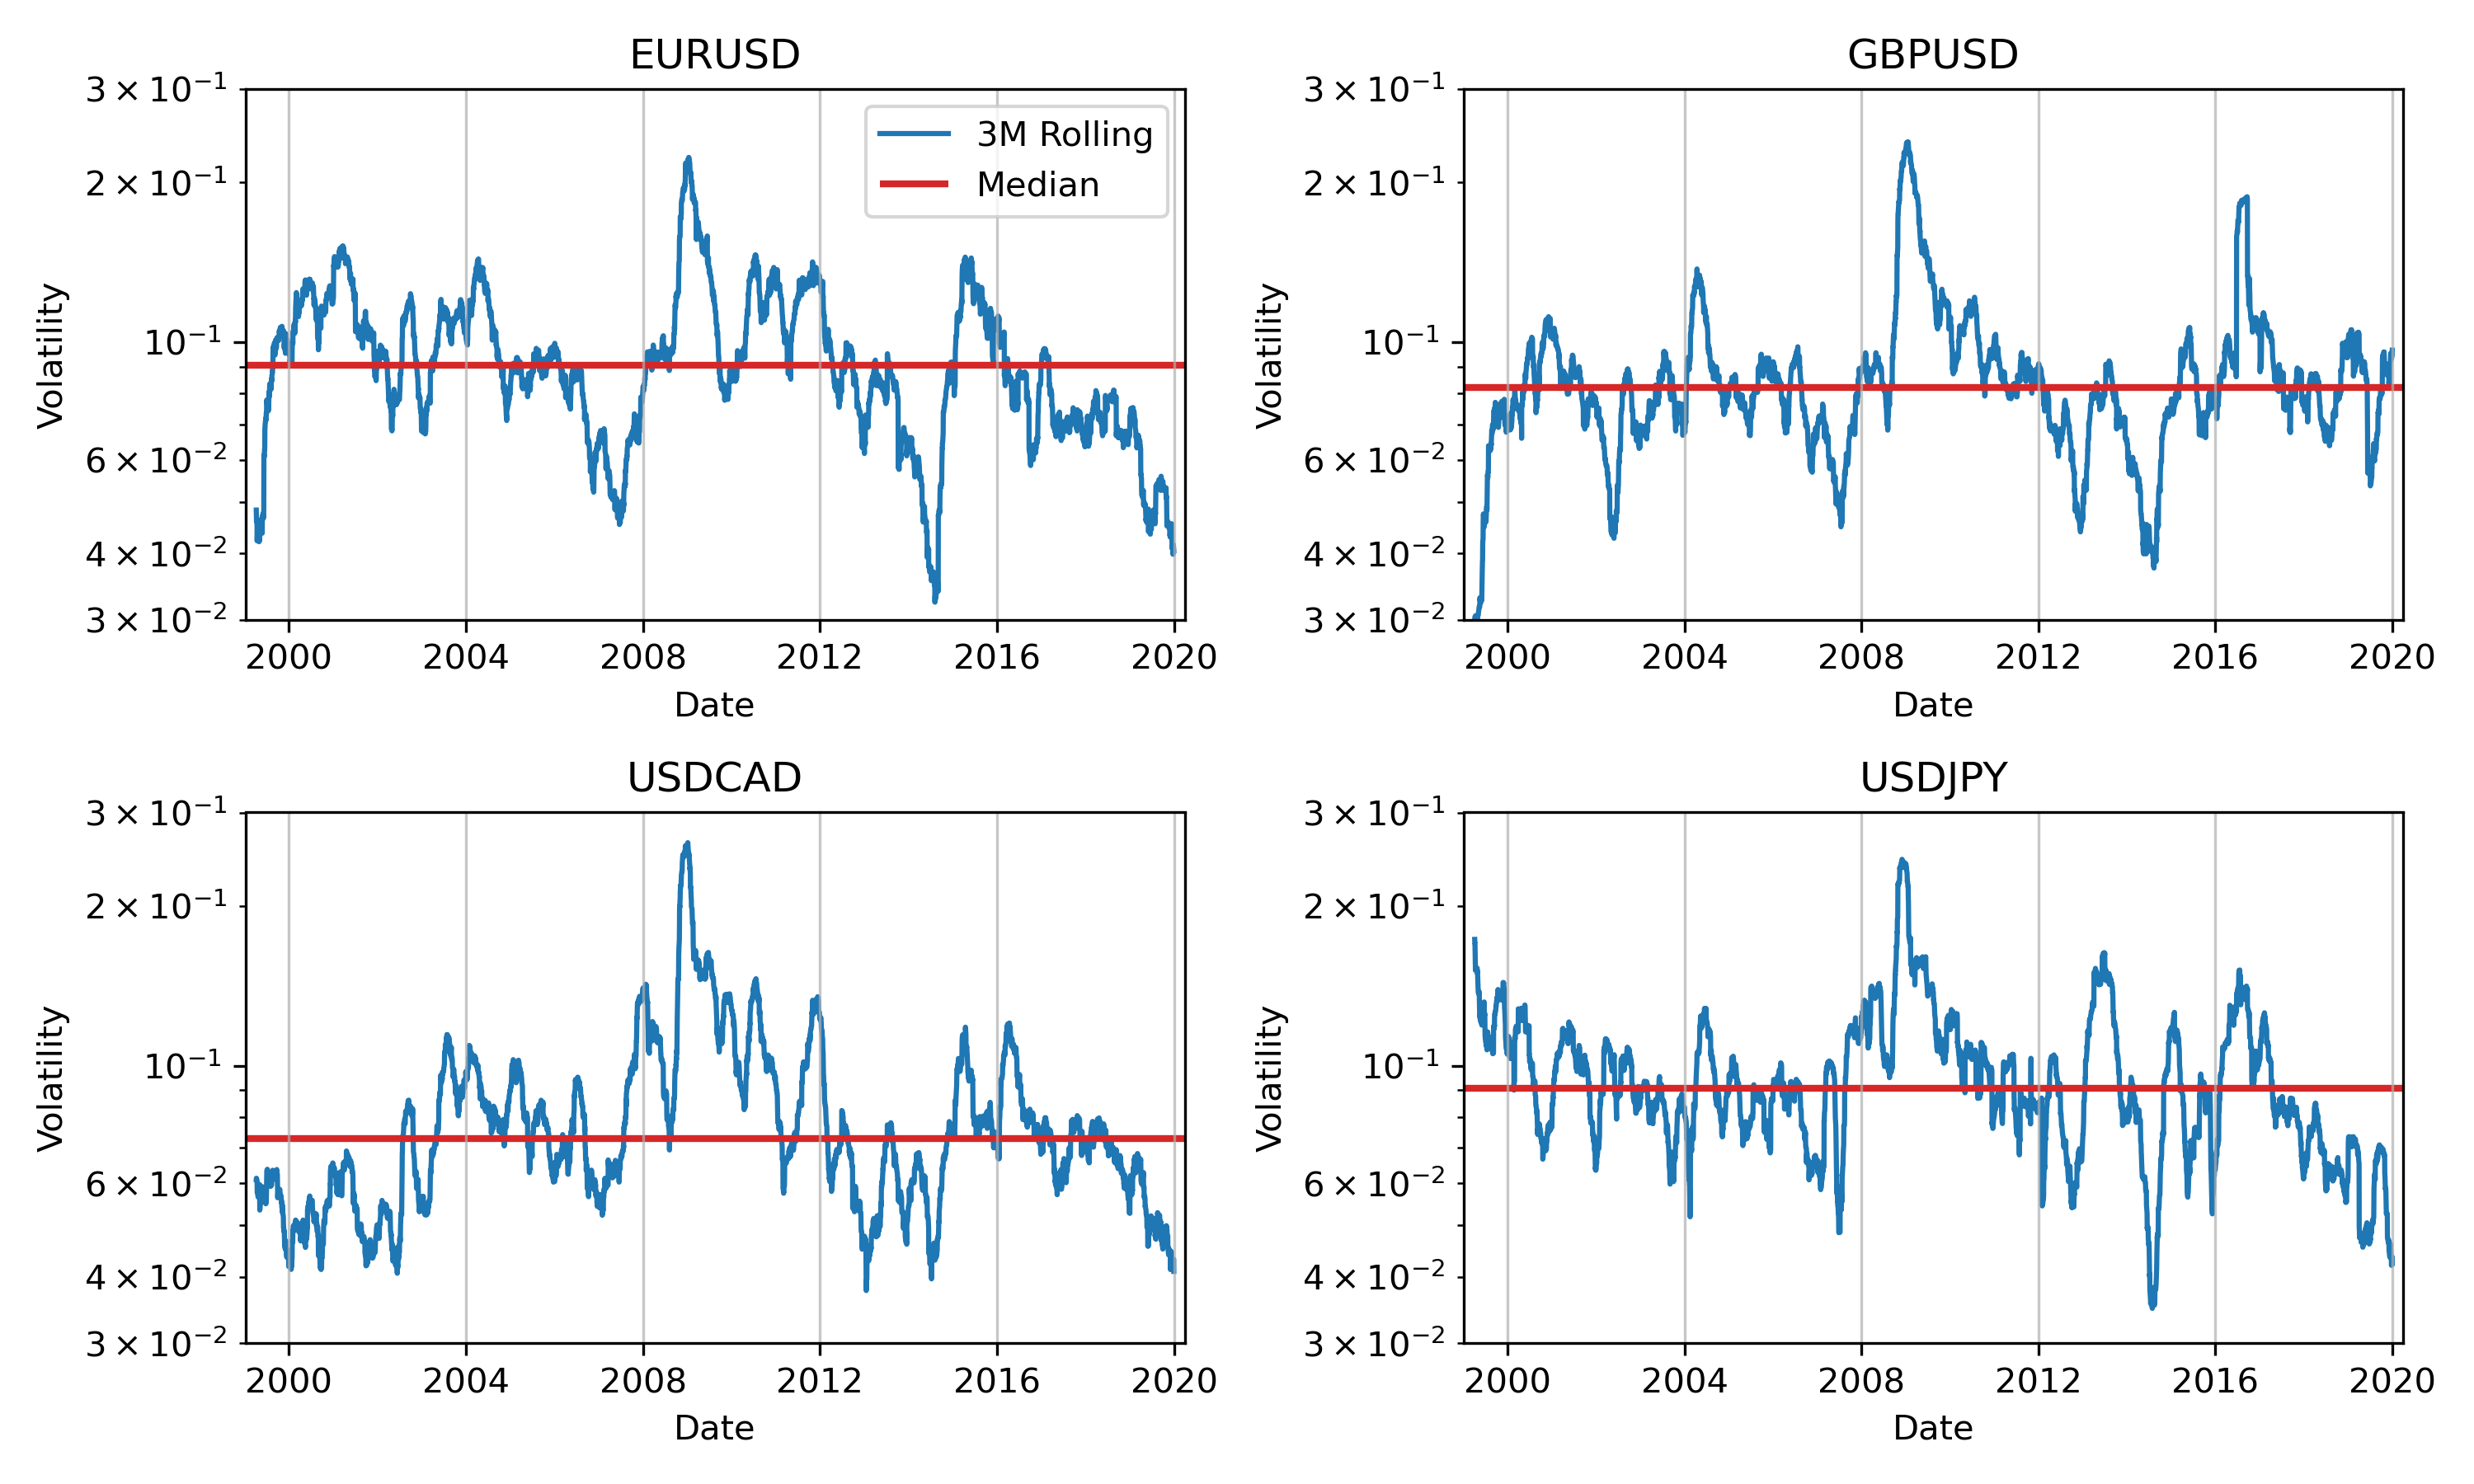
\includegraphics[width=1\linewidth]{rolling_volatility.png}
        %\label{rolling_volatilities}
    %\end{figure}
%\end{frame}

\begin{frame}
    \frametitle{Autocorrelations}
    \begin{figure}
        \includegraphics[width=1\linewidth]{autocorrelations.png}
        \label{autocorrelations}
    \end{figure}
\end{frame}

\begin{frame}
    \frametitle{QQ Plots}
    \begin{figure}
        \includegraphics[width=0.6\linewidth]{qq_032.png}
        \label{qq}
    \end{figure}
\end{frame}

\begin{frame}
    \frametitle{Correlation Coefficients}
    \begin{figure}
        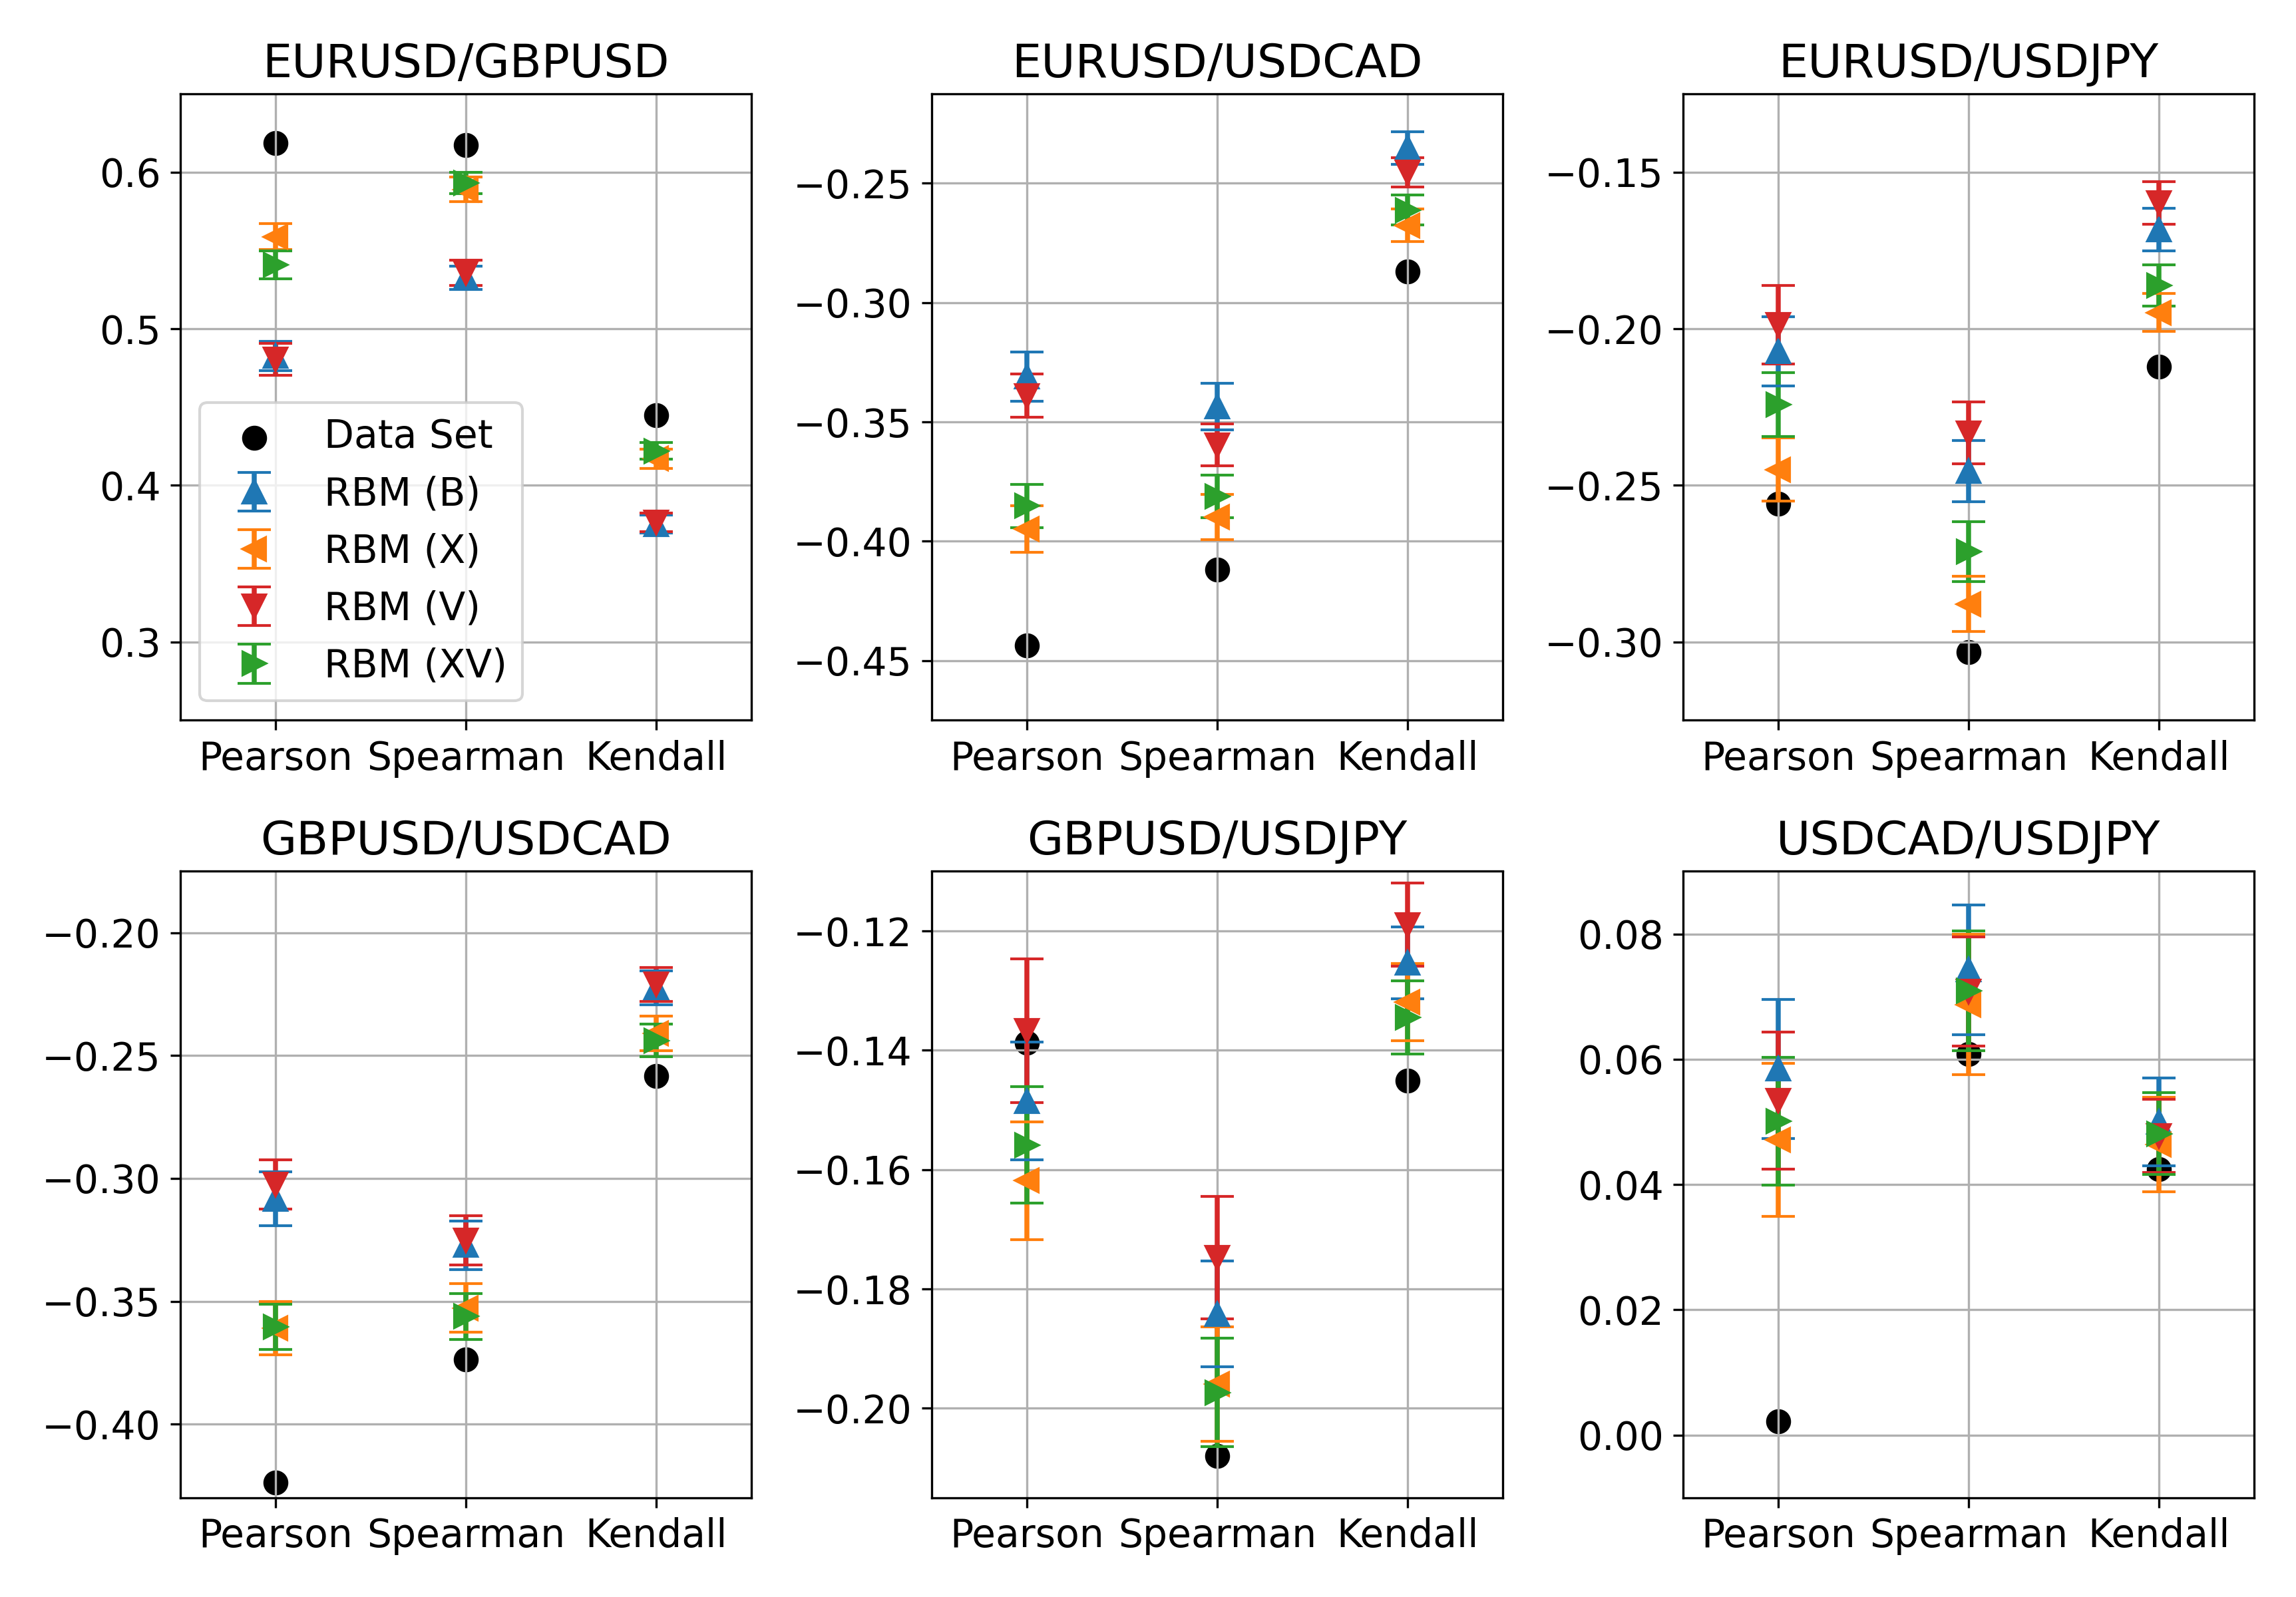
\includegraphics[width=1\linewidth]{correlation_coefficients.png}
        \label{correlation_coefficients}
    \end{figure}
\end{frame}

\begin{frame}
    \frametitle{Volatilities}
    \begin{figure}
        \includegraphics[width=0.9\linewidth]{volatilities.png}
        \label{volatilities}
    \end{figure}
\end{frame}

%----------------------------------------------------------------------------------------
% References and Resources
%----------------------------------------------------------------------------------------

\section{Next Steps}

\begin{frame}
    \frametitle{To Do}
    \begin{itemize}
        \item Improve data preprocessing/binarization to better handle outliers, e.g. try standardization as well as robust scaling before binarization.
        \item Try to understand why the full range of correlation coefficients can not be captured.
        \item Possibly incorporate other binary indicators, e.g. something to reflect the economic environment.
        \item Start working on a version of the model that can be trained/sampled using a quantum annealer.
    \end{itemize}
\end{frame}

%----------------------------------------------------------------------------------------
% References and Resources
%----------------------------------------------------------------------------------------

\section{References and Resources}

\begin{frame}[allowframebreaks]
    \frametitle{References}
    \footnotesize{
        \bibliographystyle{abbrv}
        \bibliography{../../references.bib}
    }
\end{frame}



\end{document}
